\documentclass[conference]{IEEEtran}
% The preceding line is only needed to identify funding in the first footnote. If that is unneeded, please comment it out.
\usepackage{cite}
\usepackage{amsmath,amssymb,amsfonts}
\usepackage{algorithmic}
\usepackage{graphicx}
\usepackage{textcomp}
\usepackage{xcolor}
\usepackage[acronym]{glossaries}
\usepackage{subcaption}
\usepackage[flushleft]{threeparttable}
\usepackage{booktabs}
\usepackage{adjustbox}

\usepackage{hyperref}
\usepackage{multirow}
\newcommand{\STAB}[1]{\begin{tabular}{@{}c@{}}#1\end{tabular}}


\def\BibTeX{{\rm B\kern-.05em{\sc i\kern-.025em b}\kern-.08em
    T\kern-.1667em\lower.7ex\hbox{E}\kern-.125emX}}
\begin{document}

\title{Object detection for Verification Based Annotation}
\author{\IEEEauthorblockN{Oliver Batchelor\IEEEauthorrefmark{1} and
Richard Green\IEEEauthorrefmark{2}}
\IEEEauthorblockA{Department of Computer Science,
University of Canterbury\\
Christchurch, New Zealand\\
Email: \IEEEauthorrefmark{1}oliver.batchelor@canterbury.ac.nz,
\IEEEauthorrefmark{2}richard.green@canterbury.ac.nz}}


\newacronym{VBA}{VBA}{Verification Based Annotation}
\newacronym{FCN}{FCN}{Fully Convolutional Network}
\newacronym{FPN}{FPN}{Feature Pyramid Network}


\newacronym{IID}{IID}{Independent and Identically Distributed}

\newacronym{IOU}{IoU}{Intersection over Union}
\newacronym{VOC}{VOC}{Visual Object Classes}
\newacronym{mIOU}{mIOU}{mean Intersection Over Union}

\newacronym{mAP}{mAP}{mean Average Precision}
\newacronym{AP}{AP}{Average Precision}


\newacronym{CRF}{CRF}{Conditional Random Field}

\newacronym{RELU}{ReLU}{Rectified Linear Unit}
\newacronym{PRELU}{PReLU}{Parameterised Rectified Linear Unit}
\newacronym{DECAF}{DeCAF}{Deep Convolutional Activation Feature}

\newacronym{FPN}{FPN}{Feature Pyramid Network}


\newacronym{NLL}{NLL}{Negative Loss Likelihood}
\newacronym{BCE}{BCE}{Binary Cross Entropy}
\newacronym{CE}{CE}{Cross Entropy}

\newacronym{EER}{EER}{Equal Error Rate}

 
\newacronym{COCO}{COCO}{Microsoft Common Objects in Context}
\newacronym{ILSVRC}{ILSVRC}{ImageNet Large Scale Visual Recognition Challenge}

\newacronym{NN}{NN}{Neural Network}
\newacronym{DNN}{DNN}{Deep Neural Network}

\newacronym{CNN}{CNN}{Convolutional Neural Network}
\newacronym{MCDNN}{MCDNN}{Multi-Column Deep Neural Network}

\newacronym{SSD}{SSD}{Single Shot Detector}
\newacronym{RCNN}{R-CNN}{Region CNN}

\newacronym{NMS}{NMS}{Non Maxima Suppression}


\newacronym{SIFT}{SIFT}{Scale Invariant Feature Transform}
\newacronym{SURF}{SURF}{Speeded Up Robust Features}

\newacronym{ALOI}{ALOI}{Amsterdam Library of Images}
\newacronym{MSR}{MSR}{Microsoft Research}
\newacronym{AMT}{AMT}{Amazon Mechanical Turk}

\newacronym{BOW}{BoW}{Bag of Words}
\newacronym{BOVW}{BoVW}{Bag of Visual Words}

\newacronym{ANN}{ANN}{Approximate Nearest Neighbour}
\newacronym{SGD}{SGD}{Stochastic Gradient Descent}
\newacronym{ASGD}{ASGD}{Asynchronous Stochastic Gradient Descent}
\newacronym{LOO}{LOO}{Leave One Out}

\newacronym{NCA}{NCA}{Neighbourhood Components Analysis}
\newacronym{MEGM}{MEGM}{Mean square Error's Gradient Minimisation}

\newacronym{KNN}{kNN}{k-Nearest Neighbour}

\newacronym{MSE}{MSE}{Mean Squared Error}
\newacronym{LMNN}{LMNN}{Large Margin Nearest Neighbour}
\newacronym{NCM}{NCM}{Nearest Class Mean}

\newacronym{SVM}{SVM}{Support Vector Machine}

\newacronym{PCA}{PCA}{Principle Components Analysis}
\newacronym{DRLIM}{DrLIM}{Dimensionality Reduction by Learning an Invariant Mapping}
\newacronym{SGDR}{SGDR}{Stochastic Gradient Descent with Restarts}


\newacronym{GPU}{GPU}{Graphics Processing Unit} 
\newacronym{CPU}{CPU}{Central Processing Unit}

\newacronym{API}{API}{Application Programming Interface} 

\newacronym{GHC}{GHC}{Glasgow Haskell Compiler}
\newacronym{GHCJS}{GHCJS}{GHC for JavaScript}

\newacronym{HTML}{HTML}{HyperText Markup Language}
\newacronym{SVG}{SVG}{Scaleable Vector Graphics}

\newacronym{HTTP}{HTTP}{HyperText Transfer Protocol}
\newacronym{JSON}{JSON}{JavaScript Object Notation}

\newacronym{ID}{ID}{Index of Difficulty}
\newacronym{AWS}{AWS}{Amazon Web Services}

\newacronym{CAT}{CAT}{Cumulative Annotation Time}
\newacronym{ROV}{ROV}{Remotely Operated Vehicle}


\maketitle

\begin{abstract}

In this paper we discuss several aspects of an object detector used for the purpose of online training 

\end{abstract}

\begin{IEEEkeywords}
verification, annotation, object detection, neural network, human-in-the-loop
\end{IEEEkeywords}

\section{Introduction}


\subsection{Human-in-the-loop machine learning}

\emph{Human-in-the-loop} machine learning methods are collaborations between a machine learning algorithm and a human user. The goal, where it relates to image annotation, is to make the most effective use of annotator time and reduce cognitive load. Human-in-the-loop approaches can offer improved engagement in activities that would otherwise be laborious.

Machine learning datasets often contain a lot of so-called \emph{easy} examples. These examples often dominate both the annotation process, where human time is spent needlessly annotating similar easy examples, and the learning process where the learning algorithm spends much of its computation time on examples that are already well handled. 

Human-in-the-loop machine learning includes a variety of methods. Examples include Active Learning, where an algorithm asks a human to label only the most uncertain examples, \gls{VBA} using the idea that a human annotator can recognise the correct annotation faster than manually inputting it, and \emph{interactive machine learning} where human input can be used by a machine learning algorithm to direct it, or provide hints. 

\subsection{Verification based annotation}

In this thesis, I use the term Verification Based Annotation (VBA), where machine annotations are checked and verified by a human annotator. Although the idea has played a central role in many previous works, it is not given an easily recognisable term to distinguish it from other kinds of human-in-the-loop machine learning methods such as active learning and is often conflated. A selection of verification based methods are discussed in detail below \cite{Yao2012, McNeill2011, Adhikaria2018, Castrejon2017, Papadopoulos2016, Russakovsky2015a}. 

Verification also plays a large part in ensuring consistency between human annotators in crowdsourcing efforts \cite{Su2012a}. The annotations of any one user cannot be fully trusted, and there can be significant variation between annotators. Often large organisations gamify the annotation process by having users annotate and verify labels as part of a proof-of-human process \cite{von2008recaptcha}.

Weaker algorithms (machine learning or otherwise) can be used to generate proposals which can then be validated by an annotator. An example of this is in \cite{McNeill2011} where computer vision algorithms generate proposed counts of a penguin colony, and a human operator marks false negatives and false positives.

Human verification is fast; in \cite{Papadopoulos2016}, a yes/no verification is reported as taking 1.6 seconds on average. For a full annotation of a \gls{ILSVRC} image, in \cite{Su2012a} the time to draw a bounding box is reported at 26 seconds (42 seconds after quality control), but \cite{Papadopoulos2017} reports only 7 seconds per box using a more effective input method involving clicking extremities of objects rather than selecting corners. 



\section{Method}


\subsection{Datasets}

\begin{table*}
\centering
\begin{threeparttable}
\centering
\caption{Overview of datasets, showing the variety in image and object size and number.  } 
\label{tab:resolutions} 
\begin{tabular}{llllllll}
dataset & annotations & images & box length & image size & train crop & $AP_{COCO}$ & automated \\
\toprule
$penguins$        & 7473        & 306    & $255 \pm 118$   &  $2048\times1536$  & 800                                   & 75.9  & 82.6\%                 \\
$branches$        & 2249        & 451    & $41.5 \pm 13.9$ &  $400\times400$    & 320                                   & 62.6  & 76.8\%                  \\
$seals$           & 4351        & 240    & $68.7 \pm 20.8$ &  $3920\times1600$  & 1024                                    & 80.7   & 93.4\%                 \\
$seals_b$         & 1256        & 82     & $63.4 \pm 17$   & $3920\times1600$  & 1024                                    & 72.9  & 87.3\%       \\
$scott\:base$     & 7759        & 301    & $15 \pm 3.21$     & $3927\times500$ -- $5200\times700$ & 400  & 81.4 & 84.8\%  \\
$apples^1$        & 21637       & 300    & $78.4 \pm 14.9$ &  $2592\times1728$ & 1024 & 51.8   & 75.1\%                  \\
$apples^2$        & 13418       & 168    & $92.8 \pm 11.9$ &  $3008\times2008$  & 1024                                    & 74.5  & 76.1\%                 \\
$scallops_e$      & 3669        & 6741   & $114 \pm 40.2$  &  $1280\times1024$  & 800                                   & 65.0    & 62.3\%               \\
$fisheye$         & 2598        & 367    & $96.6 \pm 32.7$ &  $2048\times1944$ & 1024                                     & 78.9   & 91.8\%                  \\
$buoys_d$         & 7221        & 207    & $38.9 \pm 42.8$ &  $1920\times1080$ & 600                                    & 70.9      & 89.9\%               \\
\shortstack{$penguin$ \\ $survey$} & 13210       & 352    & $22.6 \pm 2.11$ & $406\times405$ -- $672\times448$ & 400  & 61.6  & 89.5\%            \\ 
\bottomrule
\end{tabular}
\begin{tablenotes}
\small
\item Subscripts denote different annotators.  Datasets specified without subscript are annotated by the authors. $AP_{COCO}$ is measured on the split validation set. Box length is the length of the longest side (or diameter for circle annotations). Automated is the total proportion of annotations created from object detections without edit.

\end{tablenotes}
\end{threeparttable}
\end{table*}

\begin{figure*}[t]
\centering
\begin{subfigure}[t]{0.2\linewidth}
  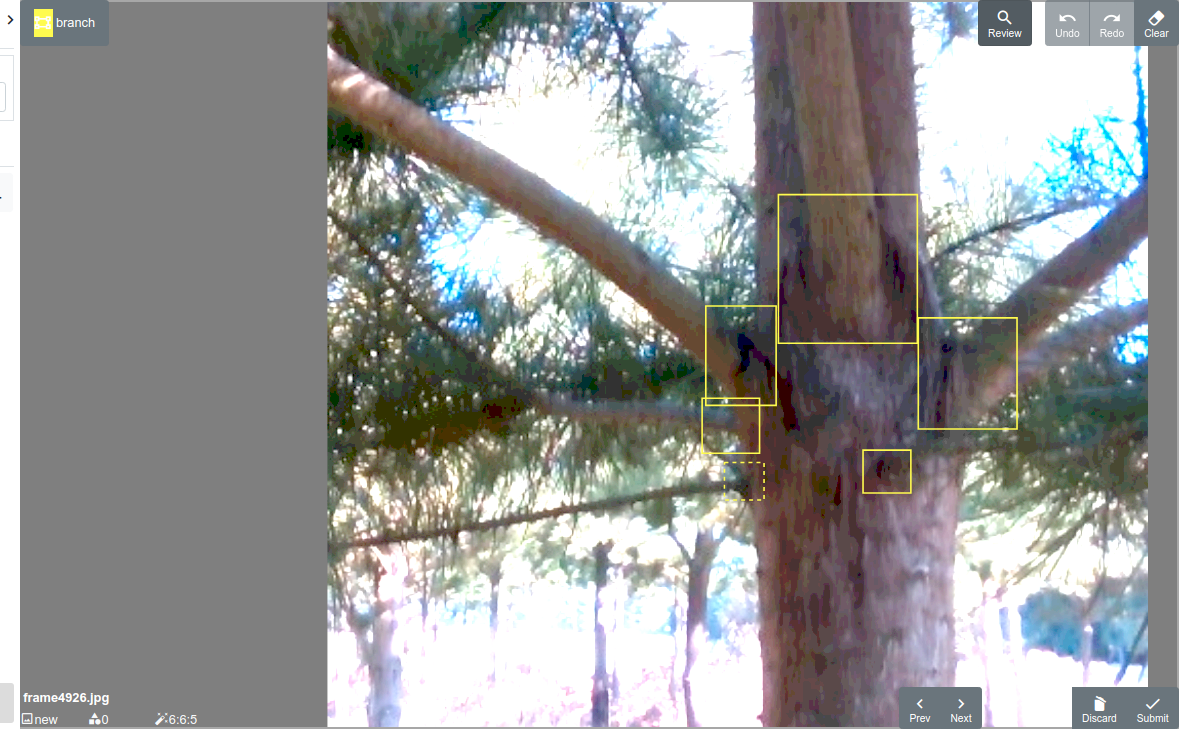
\includegraphics[width=0.9\linewidth]{figures/images/branches3.png}
   \caption{\emph{branches}}
\end{subfigure}%
\begin{subfigure}[t]{0.2\linewidth}
  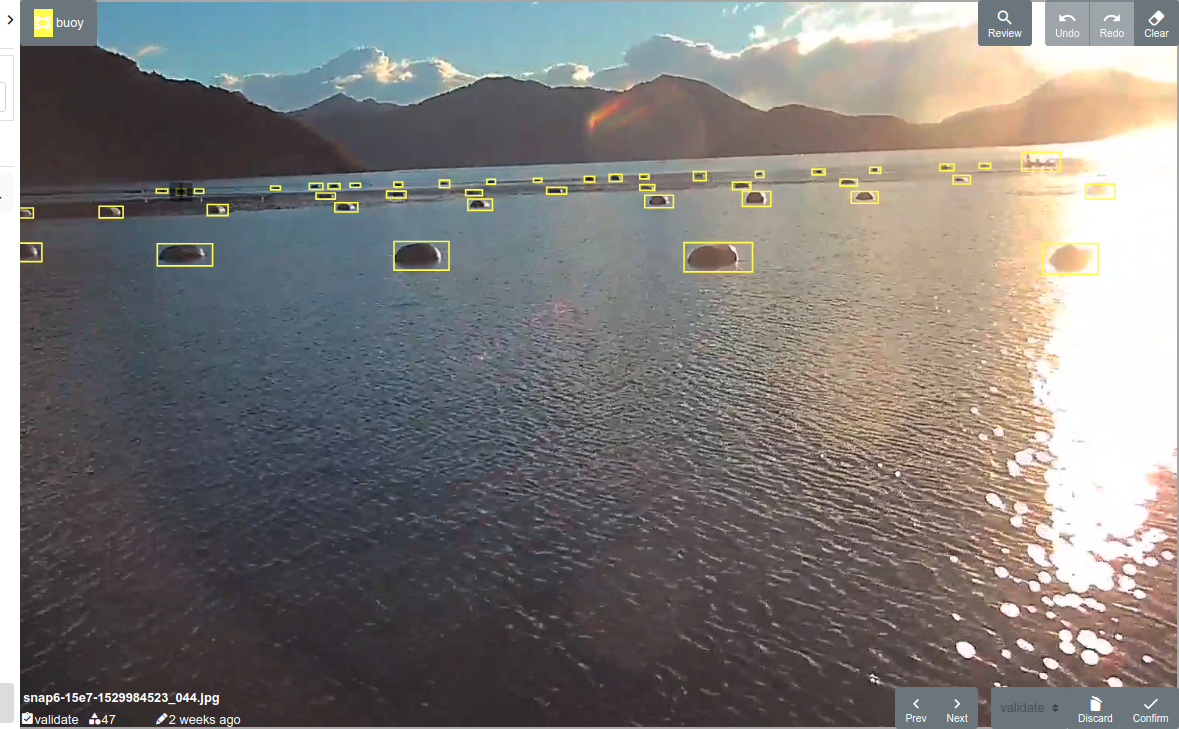
\includegraphics[width=0.9\linewidth]{figures/images/buoys.png}
   \caption{\emph{buoys}}
 \end{subfigure}%
\begin{subfigure}[t]{0.2\linewidth}
  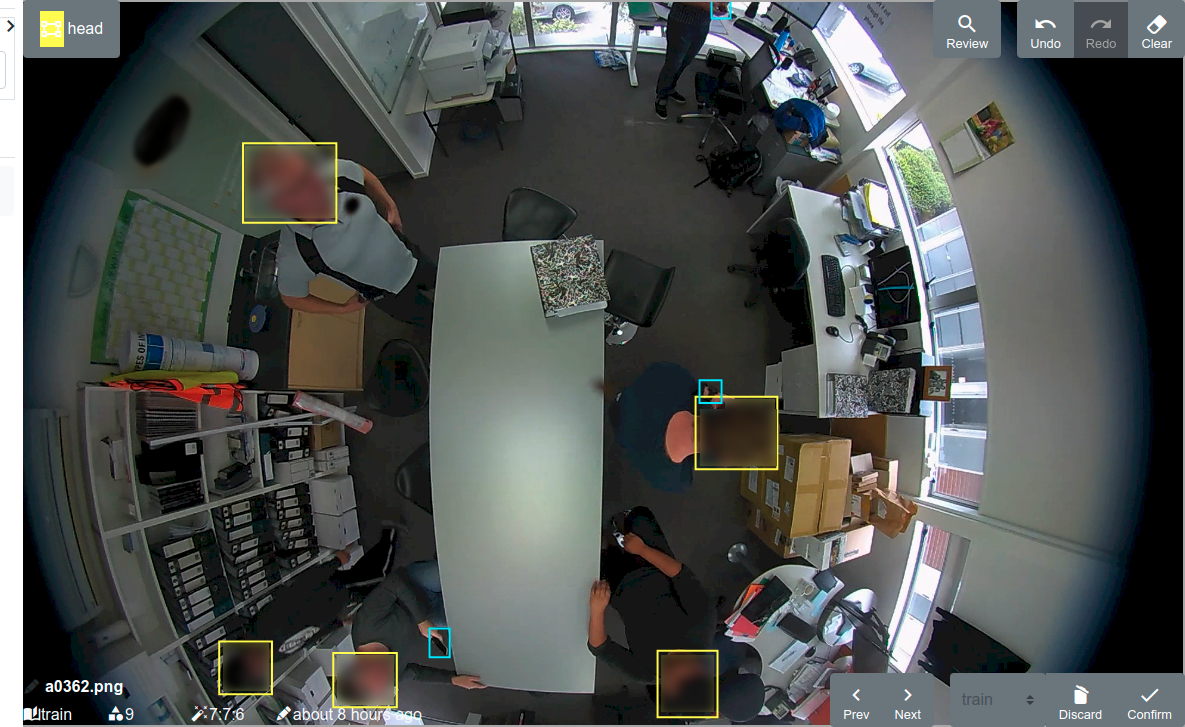
\includegraphics[width=0.9\linewidth]{figures/images/victor.png}
  \caption{\emph{fisheye}}
\end{subfigure}%
\begin{subfigure}[t]{0.2\linewidth}
  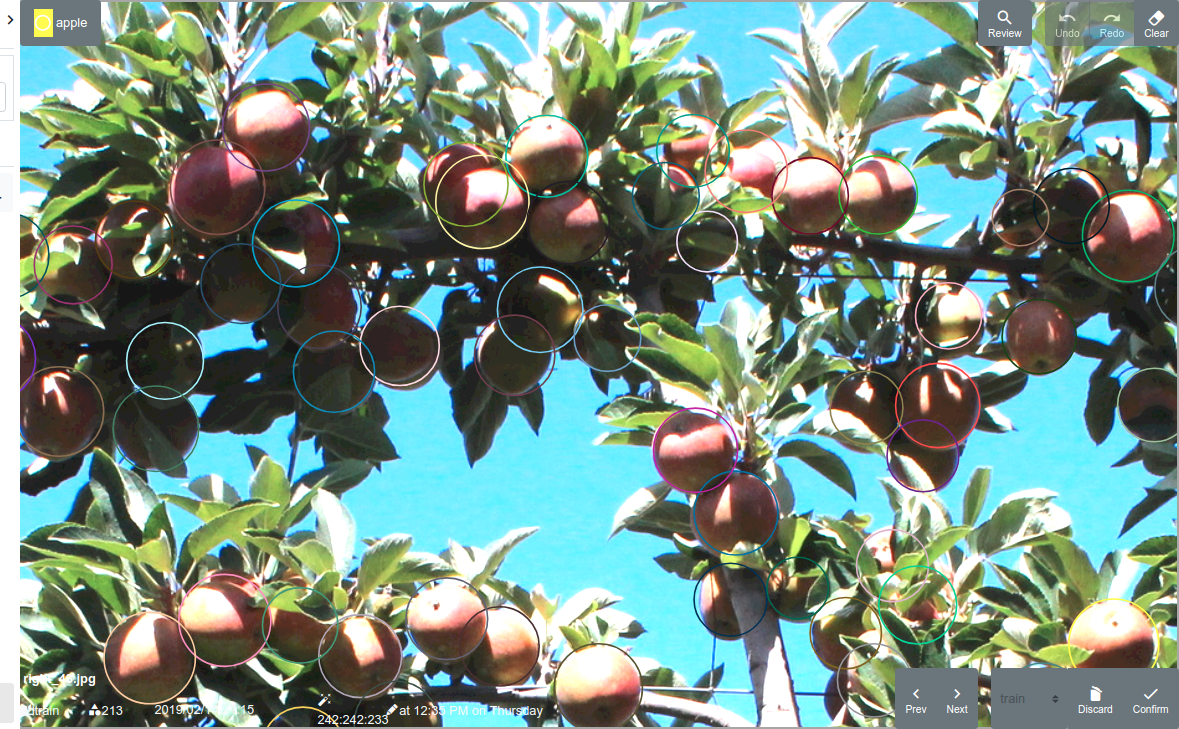
\includegraphics[width=0.9\linewidth]{figures/images/apples_big2.png}
  \caption{$\mathrm{apples_1}$}
\end{subfigure}%
\begin{subfigure}[t]{0.2\linewidth}
  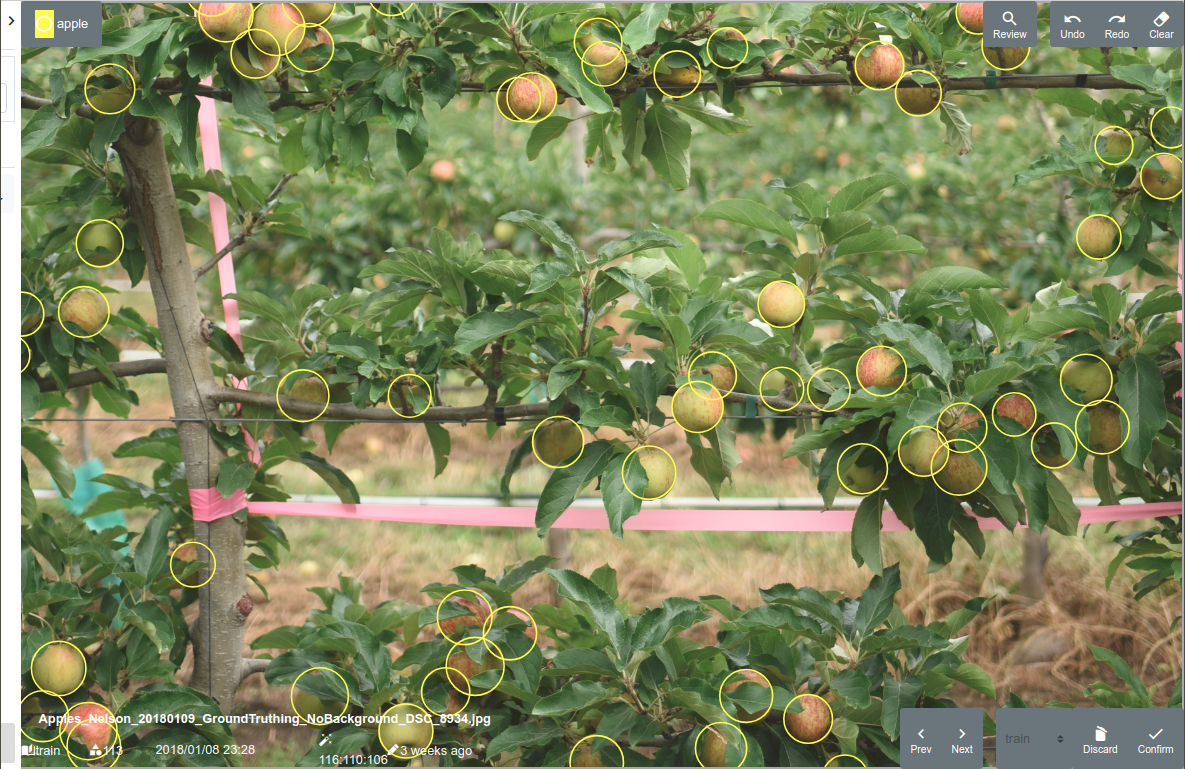
\includegraphics[width=0.9\linewidth]{figures/images/apples2.png}
  \caption{$\mathrm{apples_2}$}
\end{subfigure}
\begin{subfigure}[t]{0.2\linewidth}
  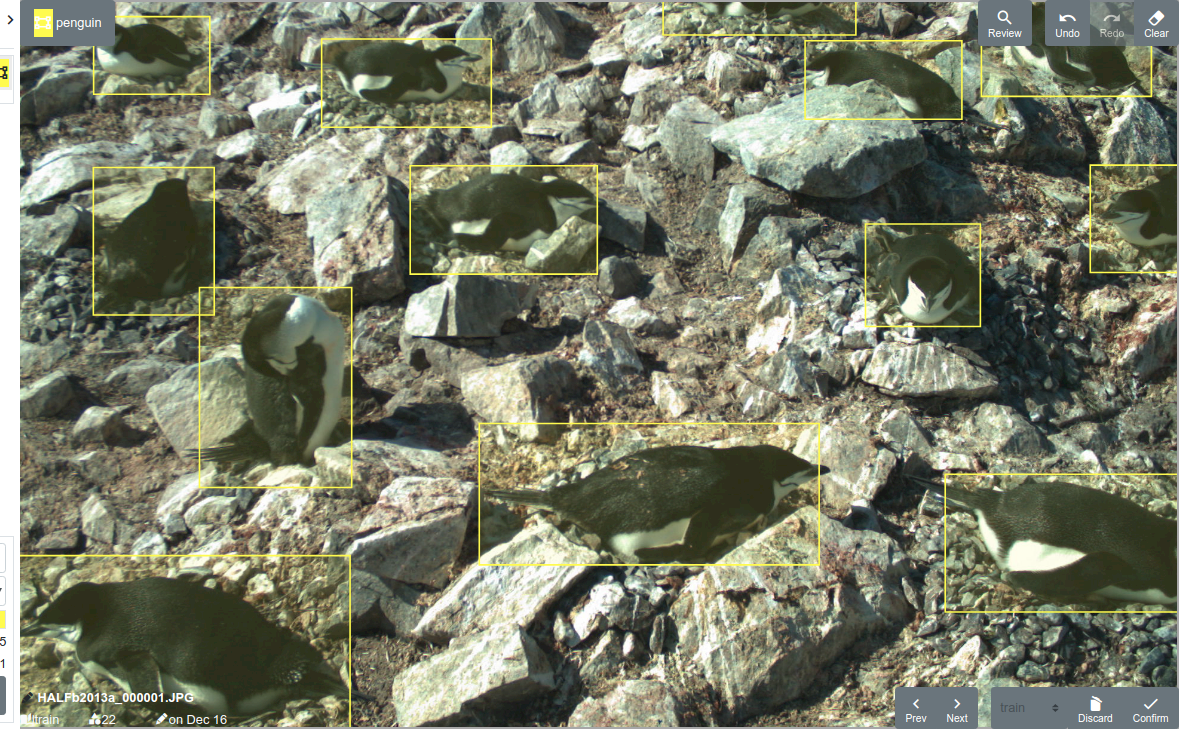
\includegraphics[width=0.9\linewidth]{figures/images/penguins2.png}
   \caption{\emph{penguins}}
\end{subfigure}%
 \begin{subfigure}[t]{0.2\linewidth}
  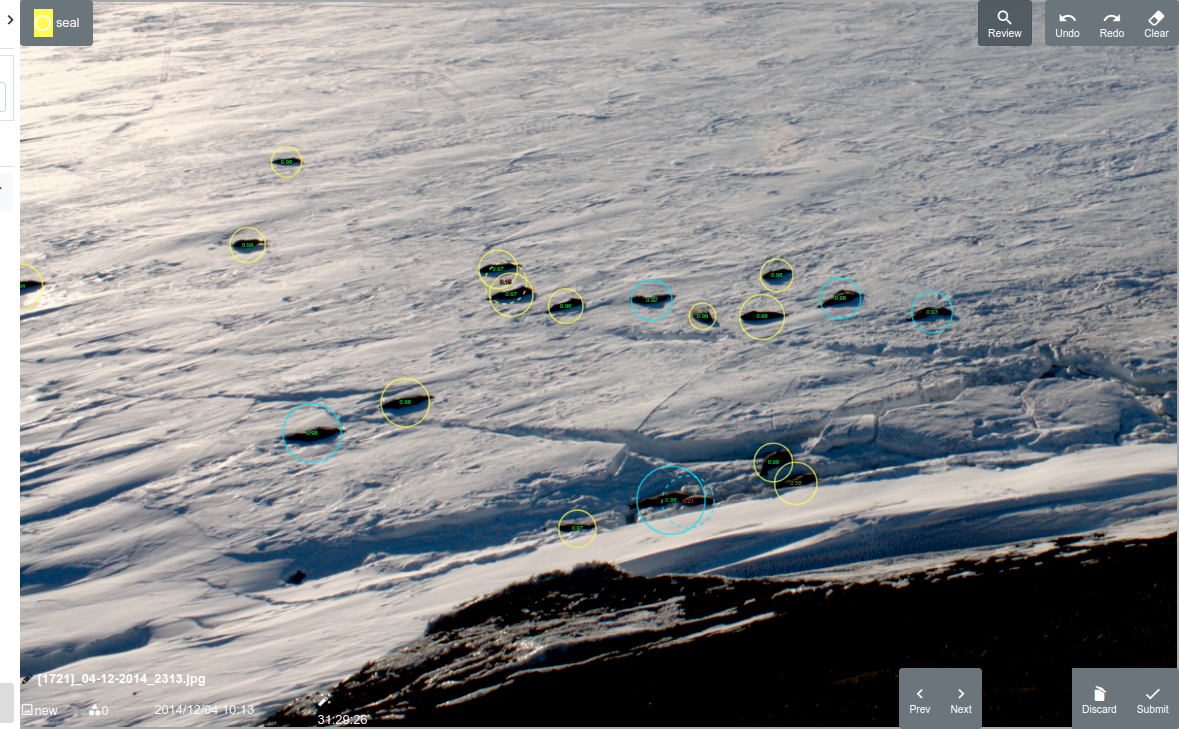
\includegraphics[width=0.9\linewidth]{figures/images/seals_small2.png}
  \caption{\emph{seals}}
\end{subfigure}%
\begin{subfigure}[t]{0.2\linewidth}
  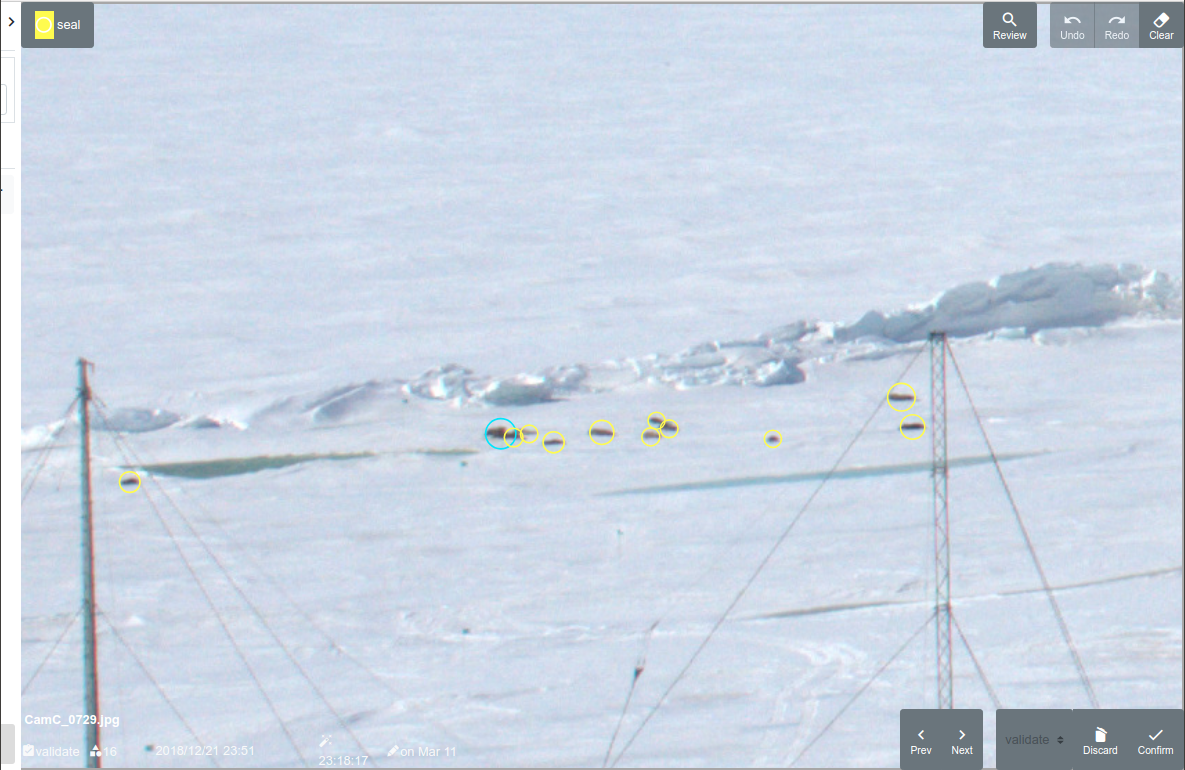
\includegraphics[width=0.9\linewidth]{figures/images/scott_base_sunny.png}
  \caption{\emph{scott base}}
\end{subfigure}%
\begin{subfigure}[t]{0.2\linewidth}
  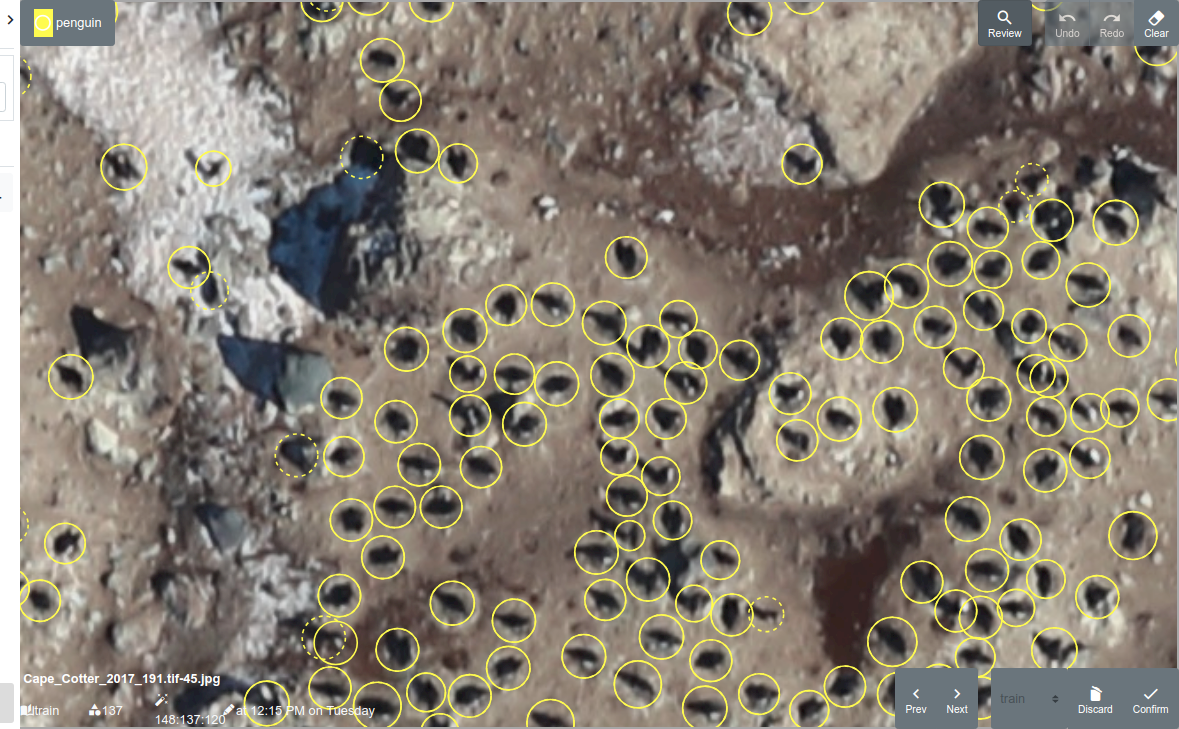
\includegraphics[width=0.9\linewidth]{figures/images/penguins_aerial2.png}
  \caption{\emph{penguin survey}}
\end{subfigure}%
\begin{subfigure}[t]{0.2\linewidth}
  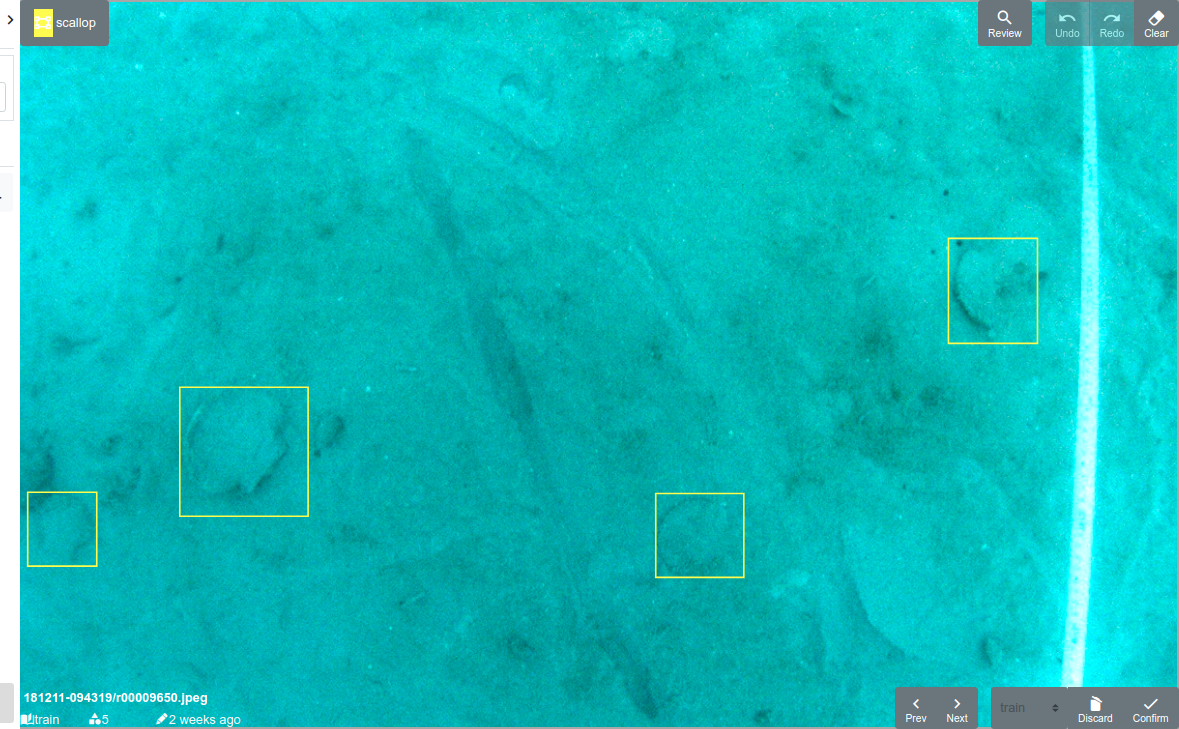
\includegraphics[width=0.9\linewidth]{figures/images/scallops4.png}
  \caption{\emph{scallops}}
\end{subfigure}
\caption{Representative images of datasets (and annotations) annotated in this work}
\label{fig:datasets_all}
\end{figure*}


\section{High resolution inference}

I looked at two different possibilities for performing inference on a full-resolution image using an object detector network trained only on crops of images: (a) pass in the full image using the property that the network is \emph{fully convolutional} and (b) tile images the same size as training crops and collapse the predictions using a combined \gls{NMS}. In order to facilitate this idea, the box annotations on the edge of images are estimates of the full bounds of the object, and the anchor boxes are not cropped to the edge of the image. In \cite{Duarte2010}, the approach of annotating the estimated full bounding box (the approach I have taken) was compared to annotating just the visible parts (as is more common practice) in a pedestrian detector. Estimating the full bounds was a slight improvement, however, the fusion of both was found to be better than either one. 

The first method is to pass in the full image to the neural network, even though it has only been trained on much smaller crops. Object detection networks are flexible and work across a range of input image resolutions. All layers are either convolutions or do not reshape the feature maps (aside from up/downsampling). As a result, passing in a larger image results in a larger feature map and set of box outputs at each layer of the pyramid. The concern is that the up/downsampling behaviour is slightly different for input sizes depending on if they are odd or even, relative to powers of two. I found this to be a legitimate concern, though largely negated if the training crop size is set to a power of two or multiple of a power of two. 

The second inference method is to tile multiple inferences at the size the model was trained at, across the full image size, using a certain overlap buffer region. The result is sets of overlapping predictions at the edges. These overlapping predictions can be decimated using a combined \gls{NMS} so that it removes duplicates overlapping from two adjacent tiles. The concern with this method is that edge detections are possibly inaccurate and may produce erroneous predictions which are not removed by \gls{NMS} because of their inaccurate localisation. 

Image size has its limits for both training and inference, as the complexity of the model and the size of the memory on the \gls{GPU} determines the maximum size image which can be processed. I can process the large images used in this work because of the relatively simple backbone model used (ResNet-18 \cite{He}). Evaluation using tiling makes it feasible to use larger image sizes and more complicated models, even if multiple inferences take more time.

\section {Incremental training}

When using the annotation tool, image annotations become available incrementally. Here I investigate the difference between training with all examples annotated up front compared to training with images added to the training set incrementally. 

During annotation, the validation set is incrementally built. Here I test against the final validation sets. In future, it would be better to use cross-validation, in order to make better use of training data, and provide more accurate testing (at the expense of extra training time). 

Figure~\ref{fig:incremental} shows the training plot for each dataset, where the validation accuracy ($AP_{COCO}$) is plotted against training time for both \emph{incremental} and \emph{full} cases. Different datasets improve at different rates with more data. However, all are restricted by the dataset size and improve with more data.

\begin{figure}[ht]
  \centering
  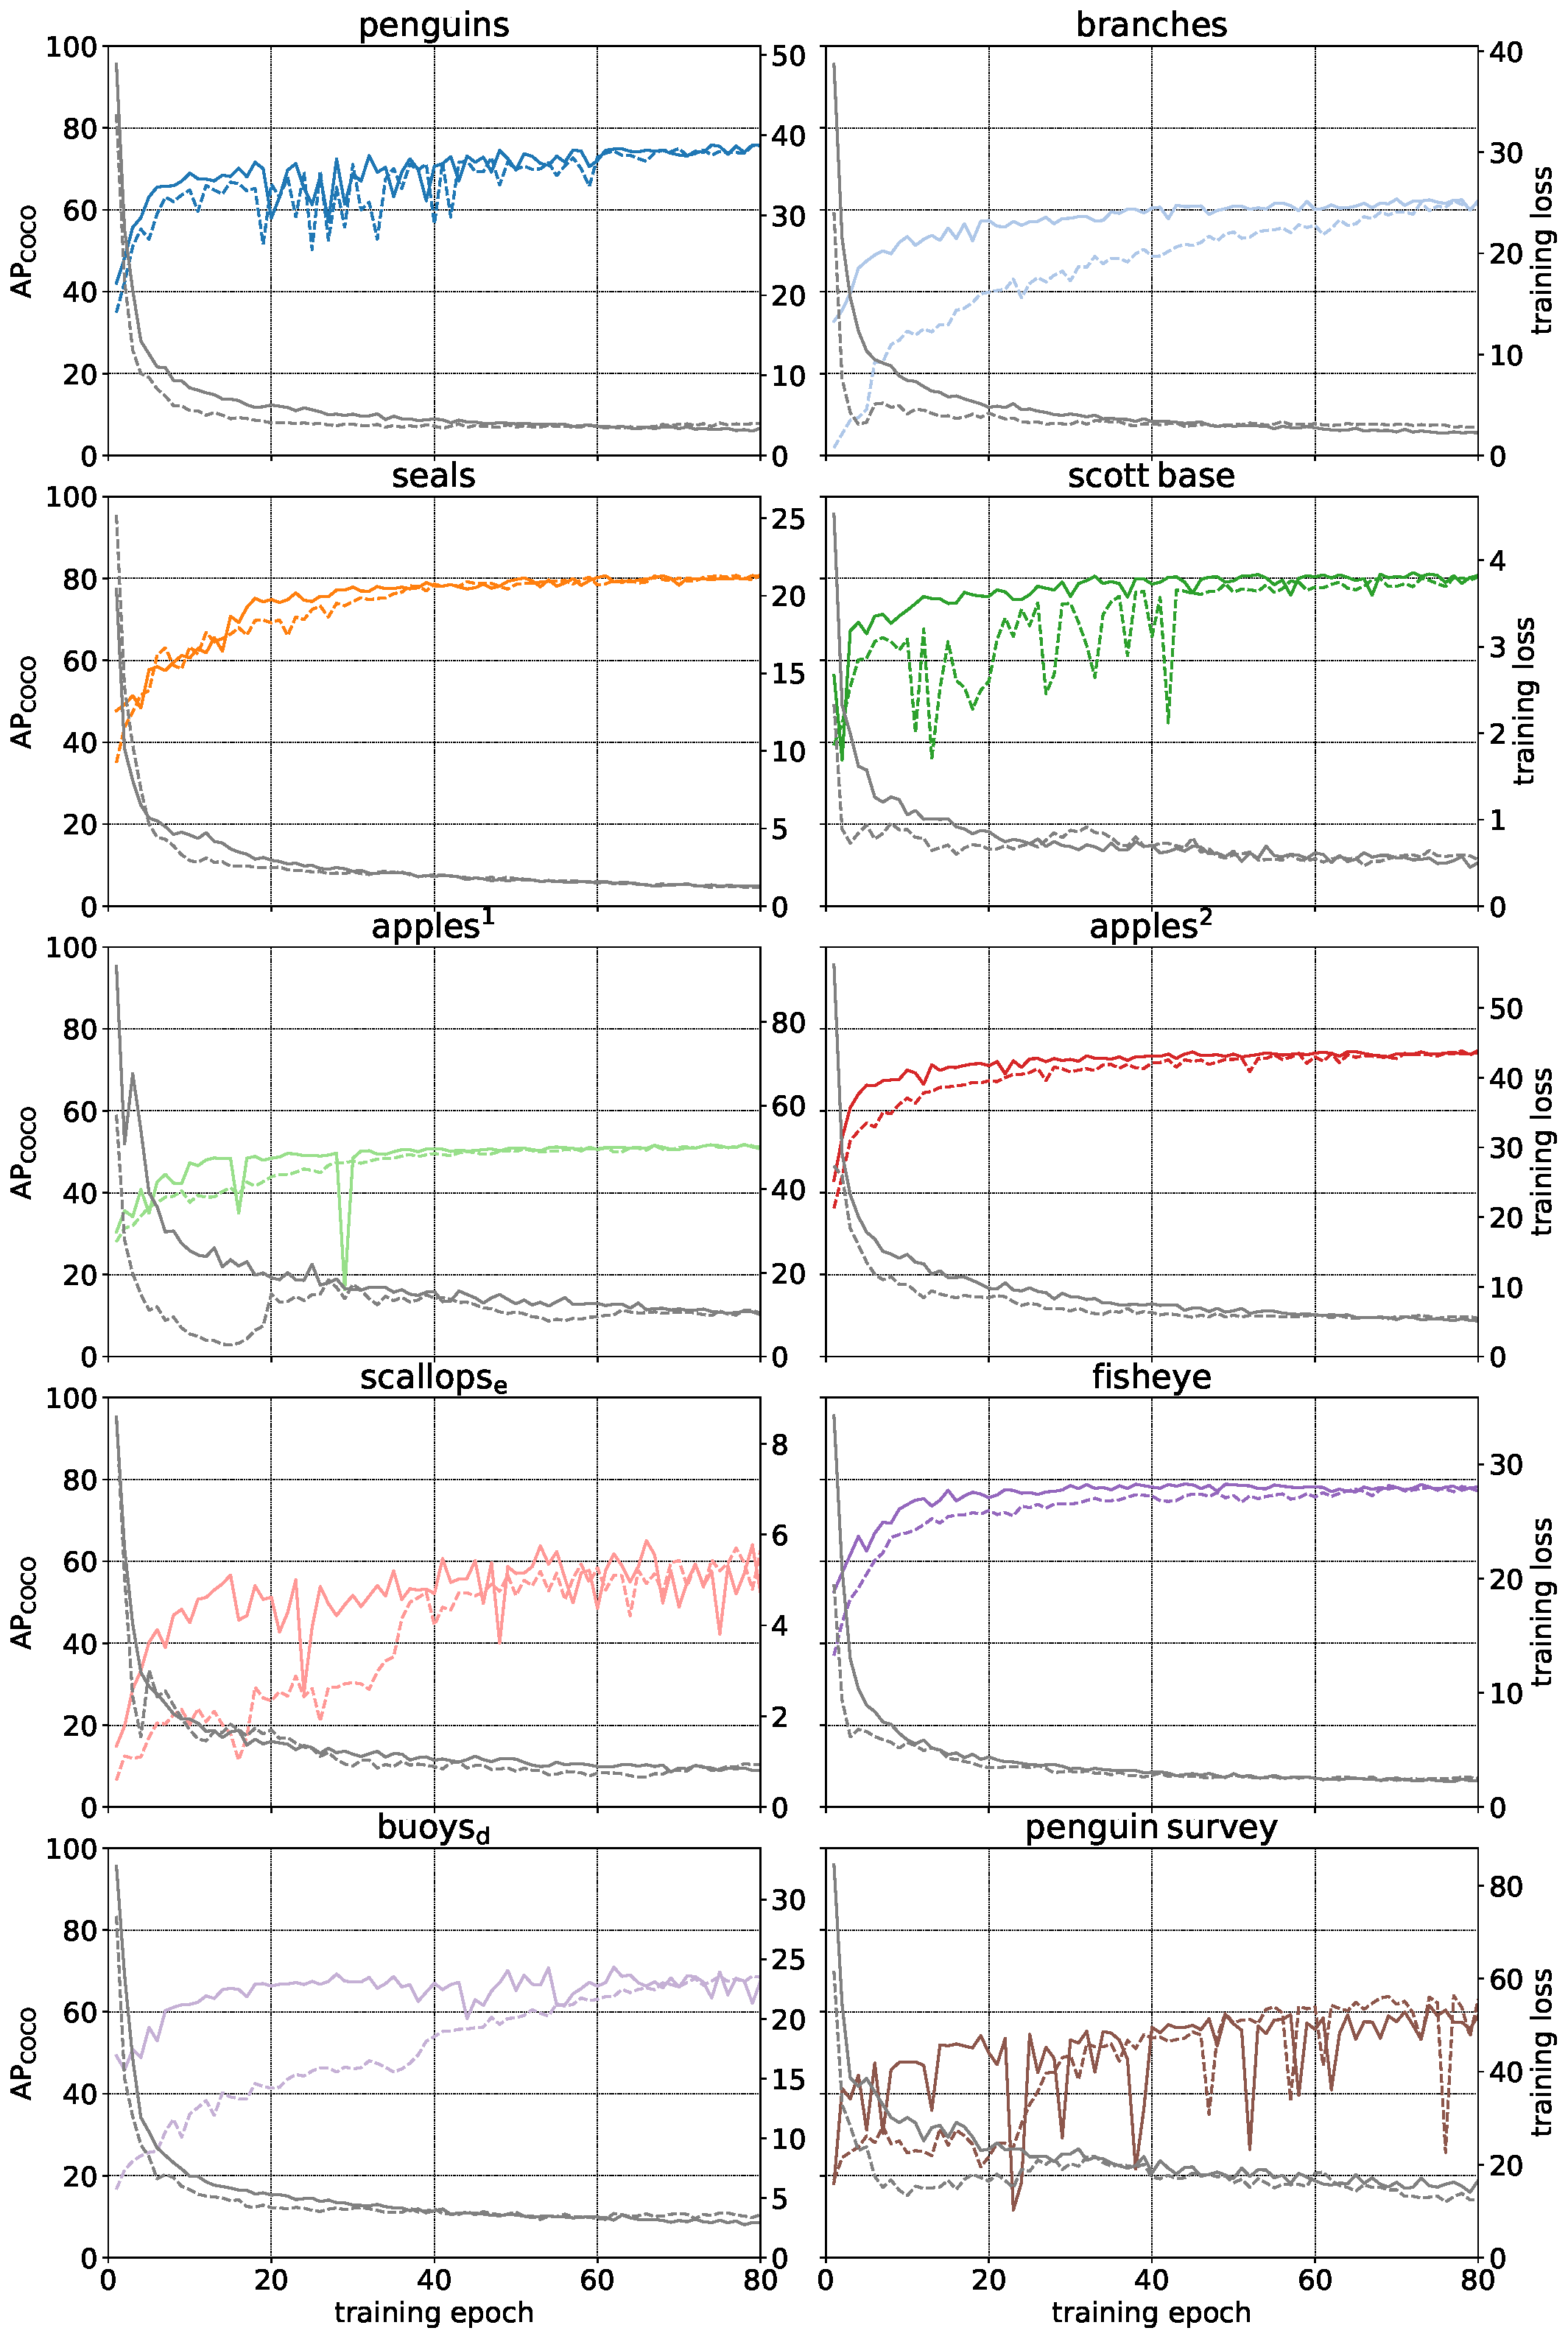
\includegraphics[width=1.0\linewidth]{figures/incremental.pdf}
  \caption{Incrementally adding examples vs. training with all examples from the beginning. Dotted lines are incremental training, solid lines are training with all examples up front. Grey lines at the bottom of each chart show the training loss.}  
  \label{fig:incremental}
\end{figure}

\section{Effect of localisation noise}

\begin{figure}[h]
\centering
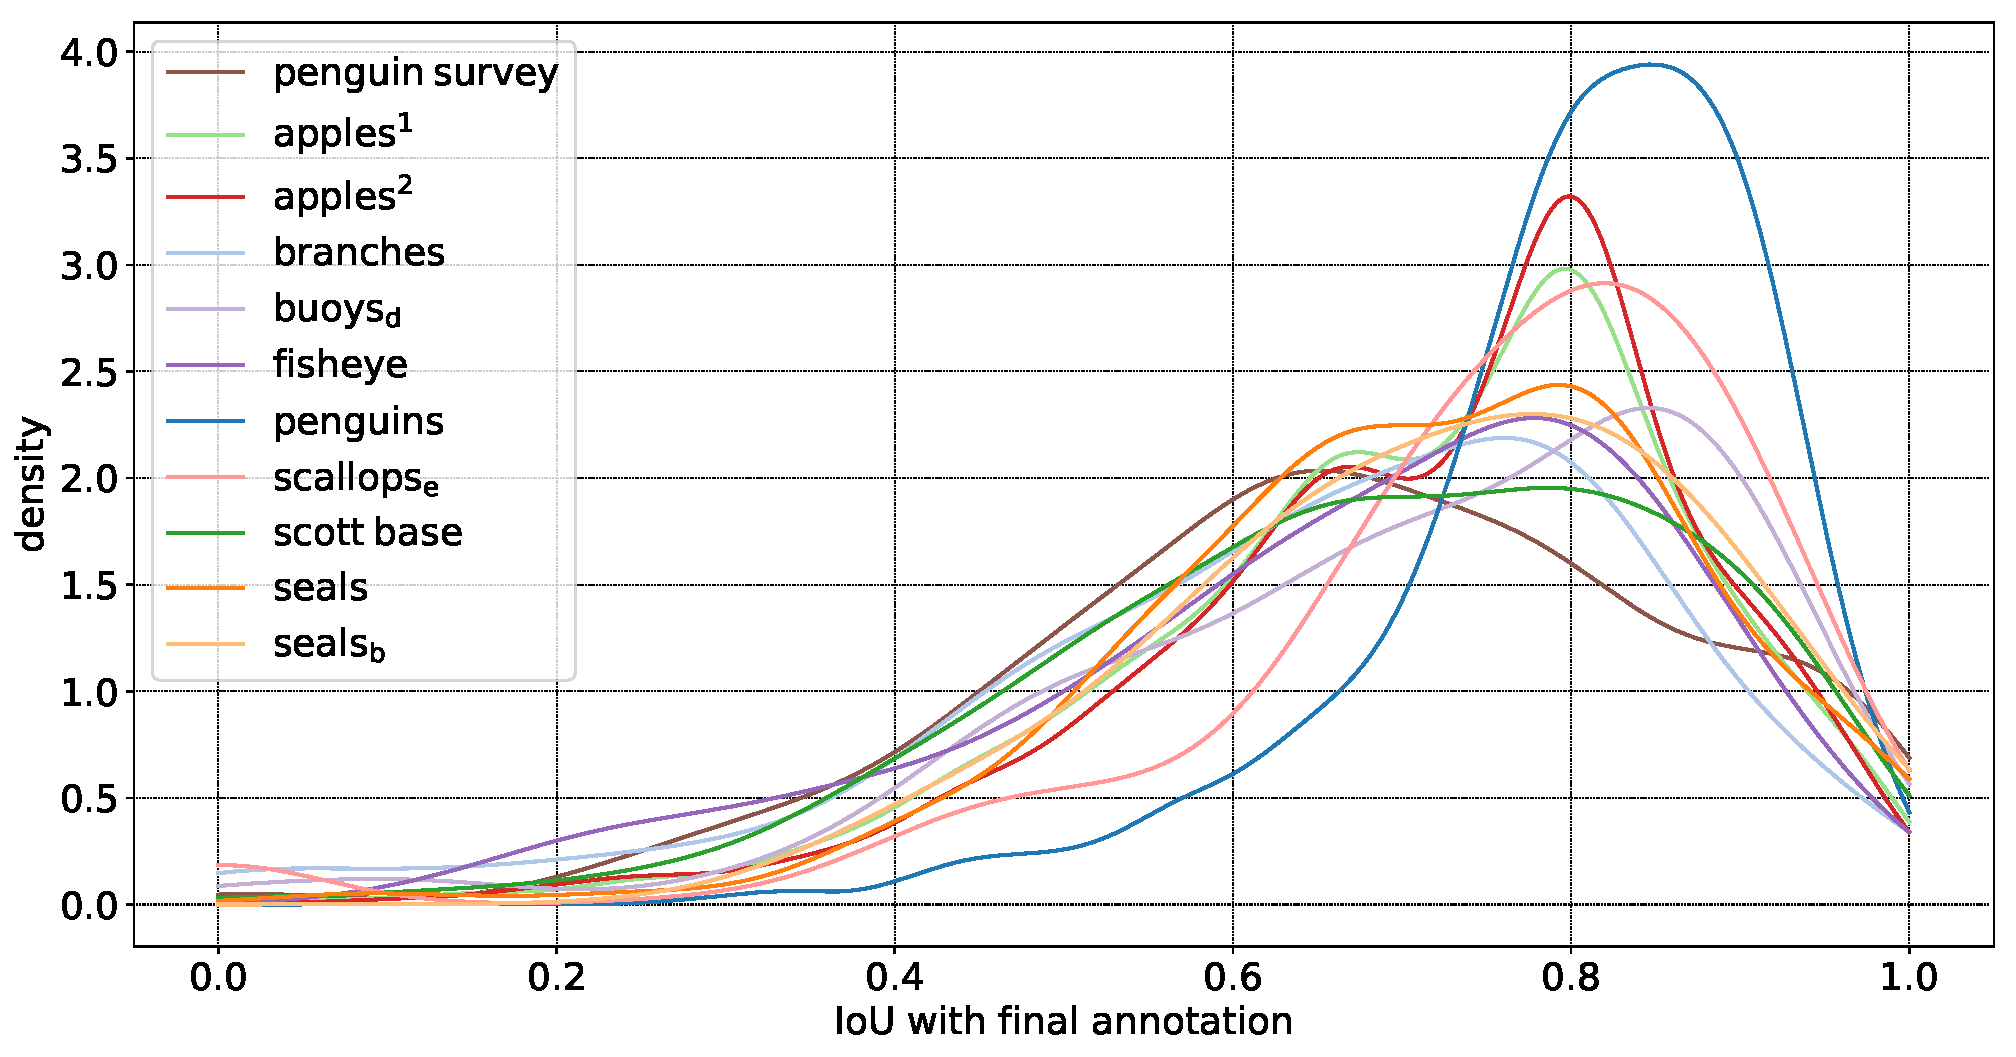
\includegraphics[width=1.0\linewidth]{figures/iou_dataset.pdf}
\caption{ Density plot of IoU overlap for detection with respect to annotation, for transformed detections. }
\label{fig:density_iou}
\end{figure}



\begin{figure}[ht]
\centering
\begin{subfigure}[t]{0.5\linewidth}
  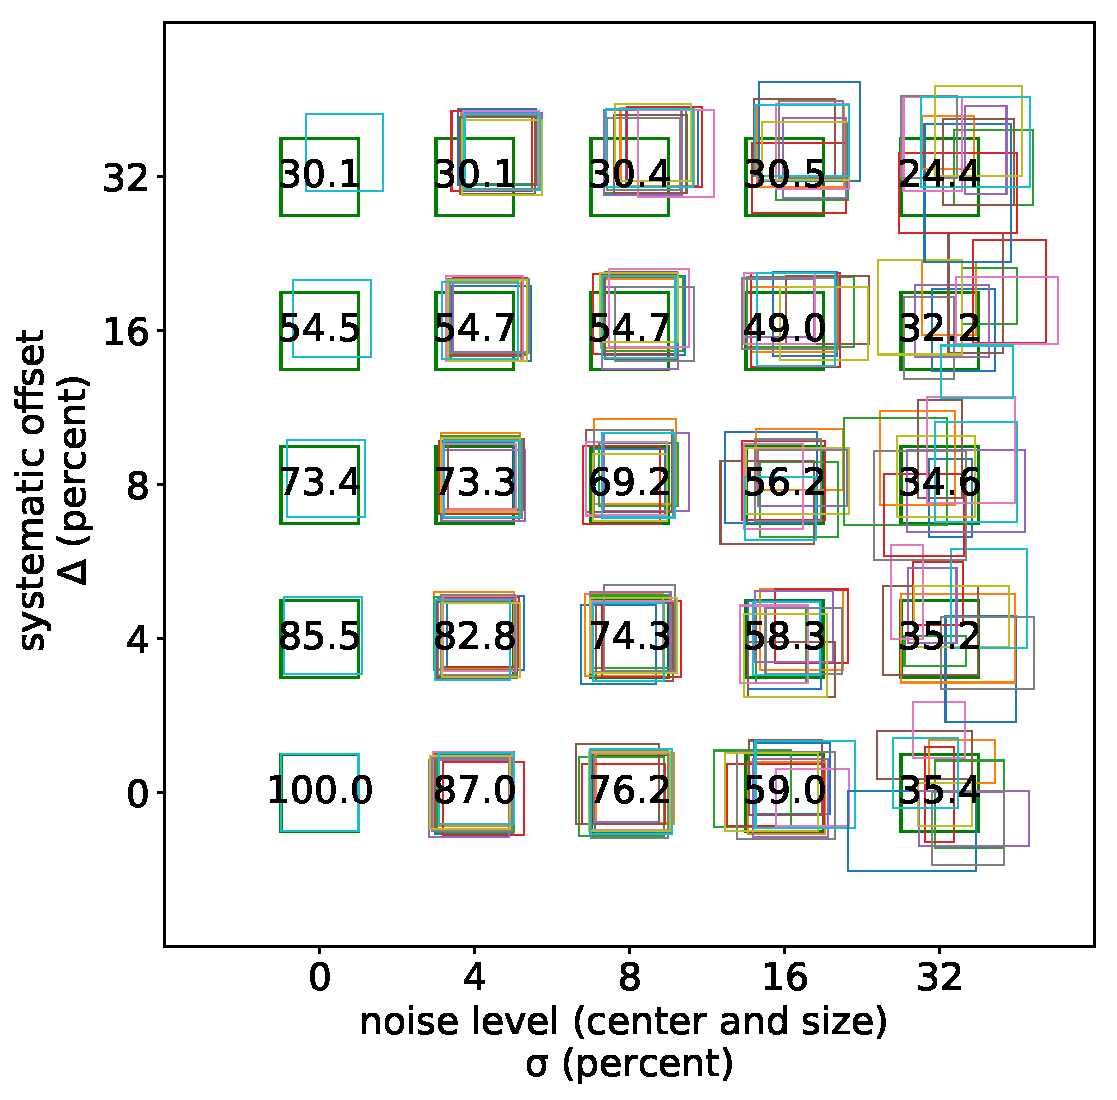
\includegraphics[width=1.0\linewidth]{figures/noisy_boxes.pdf}
  \caption{}
\end{subfigure}%
\begin{subfigure}[t]{0.5\linewidth}
  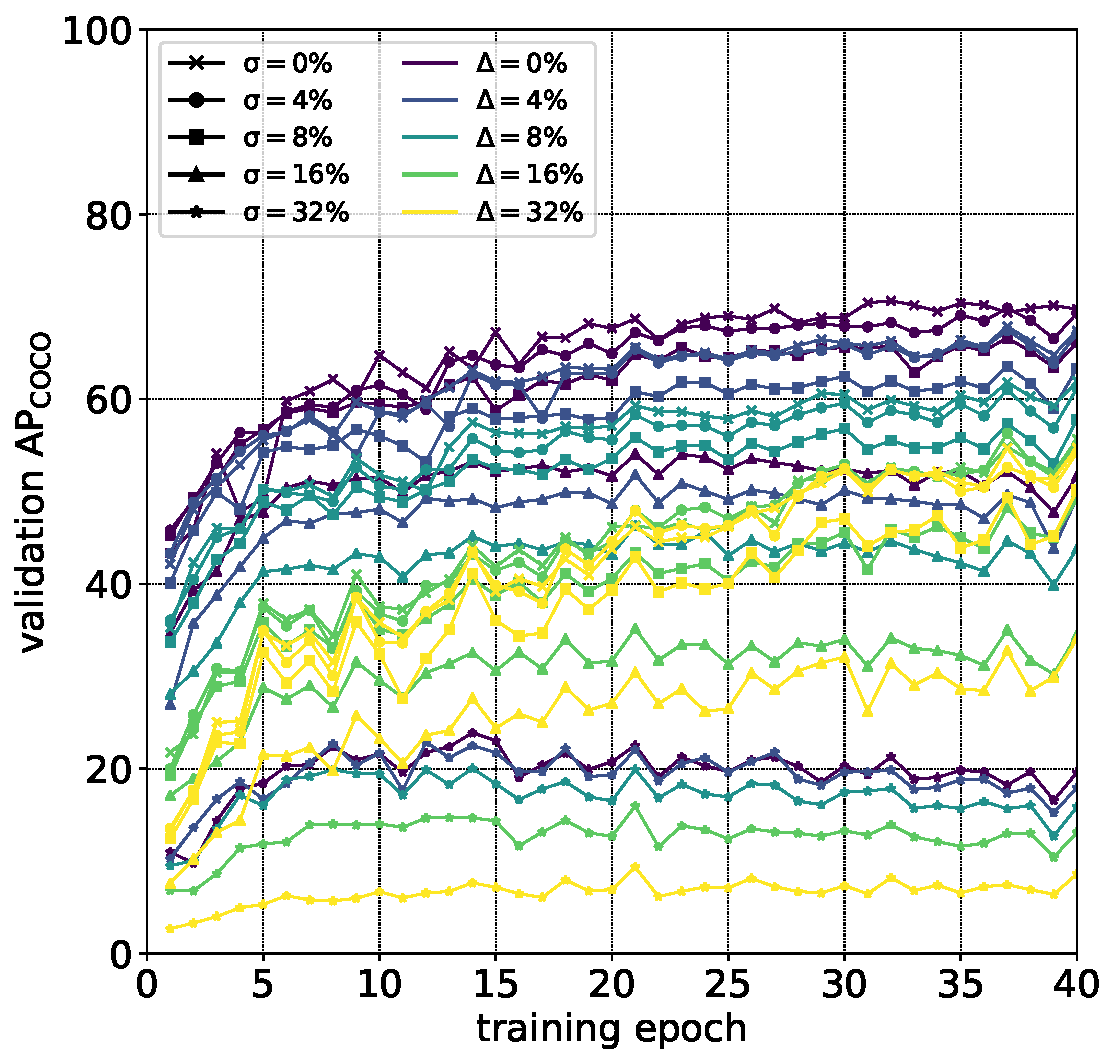
\includegraphics[width=1.0\linewidth]{figures/noise_training.pdf}
  \caption{100\% training images}
\end{subfigure}
\begin{subfigure}[t]{0.5\linewidth}
  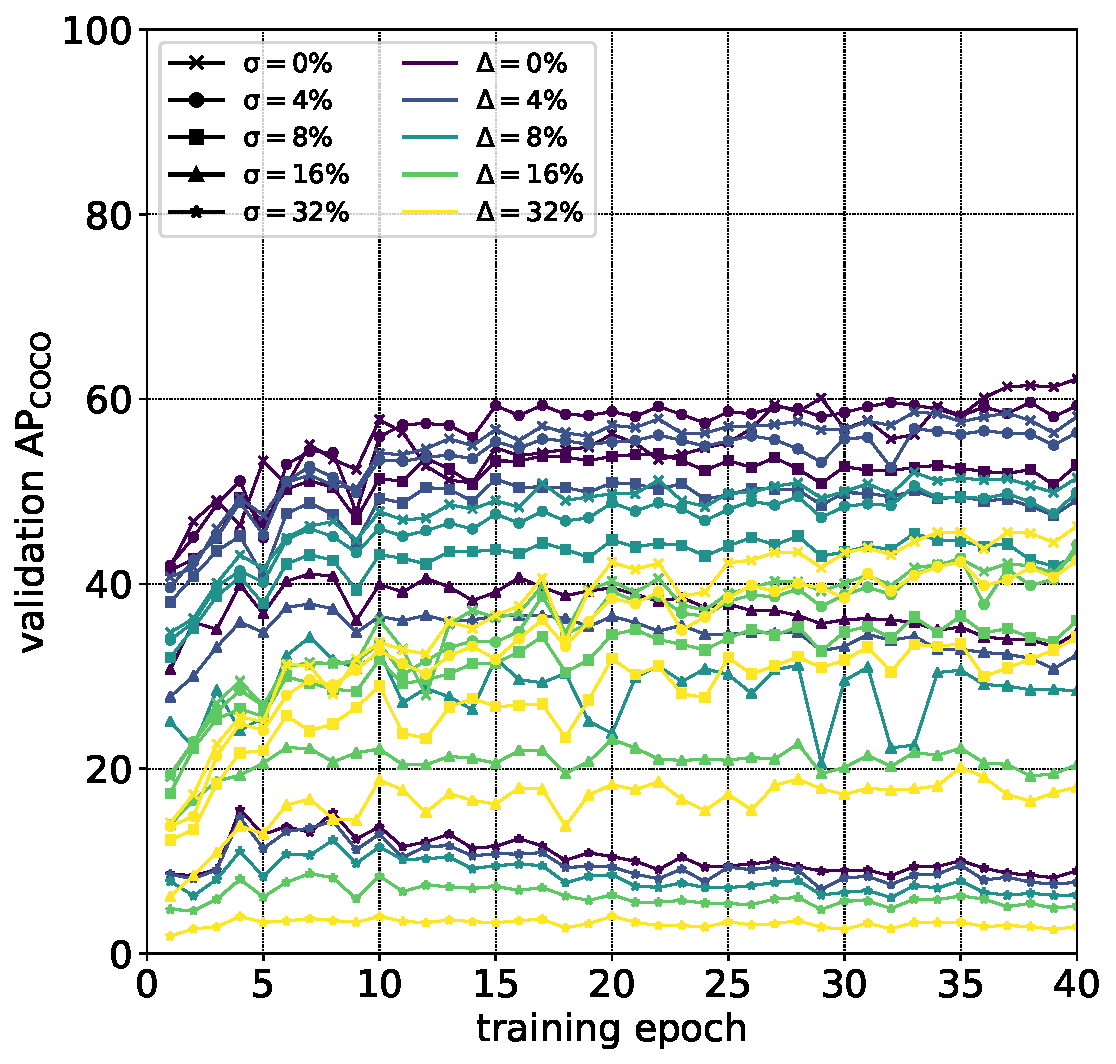
\includegraphics[width=1.0\linewidth]{figures/noise_4_training.pdf}
  \caption{25\% training images}
\end{subfigure}%
\begin{subfigure}[t]{0.5\linewidth}
  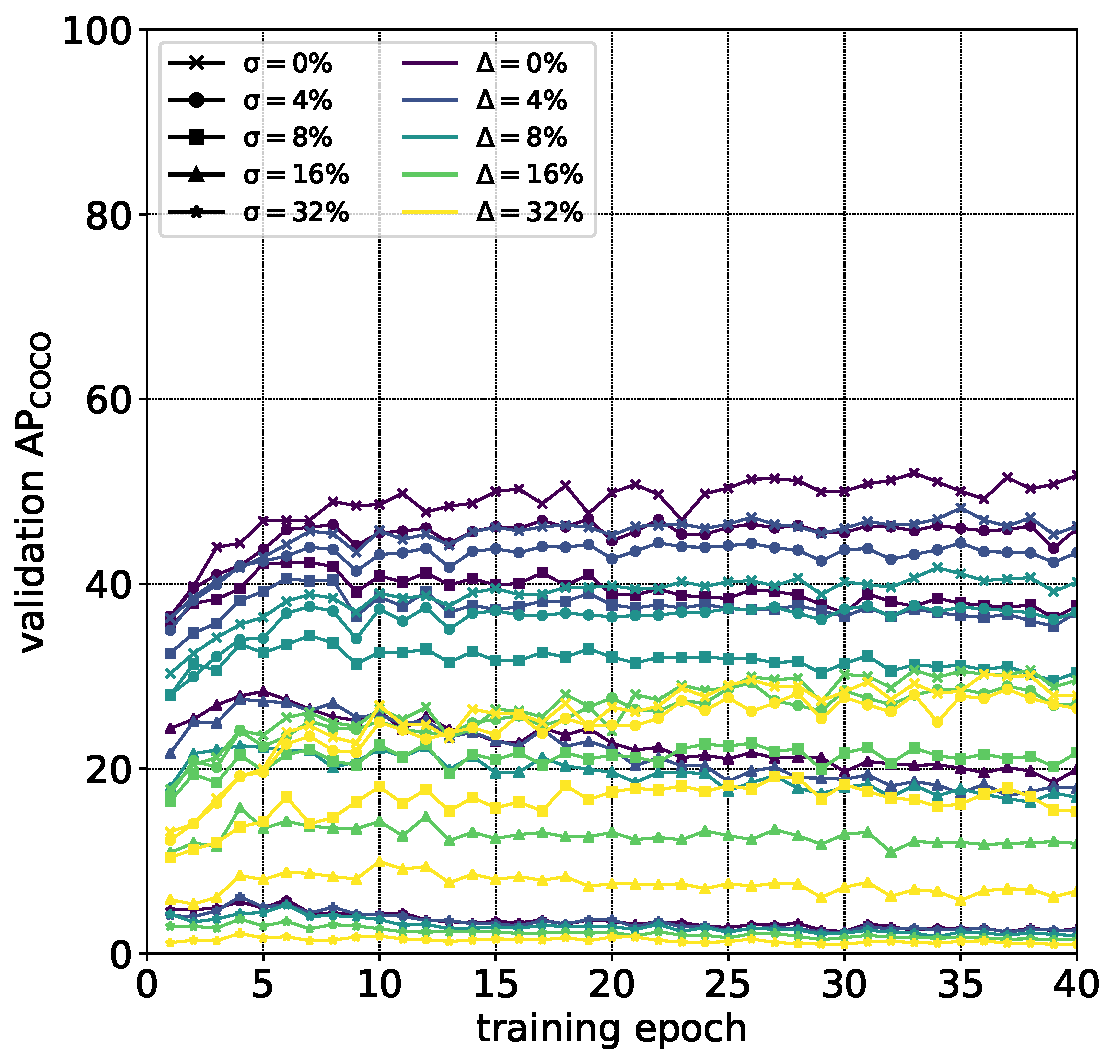
\includegraphics[width=1.0\linewidth]{figures/noise_16_training.pdf}
  \caption{6.25\% training images}
\end{subfigure}
  \caption{ (a) Samples of the different noise and systematic bias added, showing reference box with 10 samples; overlaid with the mean \gls{IOU} for that condition. (b), (c), (d) $AP_{COCO}$ validation after training with with varying noise and systematic bias added, and varying training set size. Average of training runs of 5 different datasets, at half-resolution: \emph{seals}, $apples^2$ and \emph{penguins}; at full-resolution: \emph{scott base}, \emph{branches}}
  \label{fig:noisy_training}
\end{figure}


\begin{table}[]
\caption {Best validation $AP_{50}$, $AP_{75}$, with different levels of added noise ($\sigma$) and systematic bounding box offset ($\Delta$) and at different sizes of training data. Baseline ($\sigma=0$, $\Delta=0$) in each case shown as absolute value in bold, other cases shown as percent change. Mean and standard deviation of 5 different datasets, at half-resolution: \emph{seals}, $apples^2$ and \emph{penguins}; at full-resolution: \emph{scott base}, \emph{branches}.}
\label{tab:noise_table}


\begin{subfigure}[b]{\linewidth}
\caption{$100\%$ training data}
\begin{adjustbox}{max width=\textwidth}
\begin{tabular}{ll|lllll}
 & & $\Delta=0\%$              & $\Delta=4\%$              & $\Delta=8\%$              & $\Delta=16\%$              & $\Delta=32\%$              \\

\toprule
\multirow{2}{*}{\STAB{\rotatebox[origin=c]{90}{$AP_{50}$}}}
 & $\sigma=0\%$  & $\mathbf{95.1\pm2.7}$  & $-0.6\pm0.6\%$  & $-0.7\pm0.7\%$  & $-2.8\pm2.1\%$  & $-10.1\pm10.6\%$ \\
 & $\sigma=4\%$  & $-0.3\pm0.6\%$  & $-0.4\pm0.6\%$  & $-1.3\pm1.4\%$  & $-2.8\pm1.7\%$  & $-10.4\pm10.3\%$ \\
 & $\sigma=8\%$  & $-1.1\pm0.8\%$  & $-1.3\pm1.7\%$  & $-2.4\pm1.5\%$  & $-4.0\pm2.3\%$  & $-12.6\pm9.8\%$  \\
 & $\sigma=16\%$ & $-6.9\pm4.7\%$  & $-8.4\pm5.3\%$  & $-8.0\pm4.4\%$  & $-10.2\pm3.7\%$ & $-23.8\pm11.7\%$ \\
 & $\sigma=32\%$ & $-32.6\pm6.8\%$ & $-32.1\pm7.1\%$ & $-36.1\pm4.4\%$ & $-42.2\pm4.8\%$ & $-61.5\pm6.6\%$ \\

\toprule
\multirow{2}{*}{\STAB{\rotatebox[origin=c]{90}{$AP_{75}$}}}
 & $\sigma=0\%$  & $\mathbf{84.0\pm8.5}$   & $-2.7\pm1.5\%$   & $-9.1\pm3.4\%$   & $-27.3\pm21.5\%$ & $-24.1\pm17.0\%$ \\
 & $\sigma=4\%$  & $-2.1\pm1.1\%$   & $-2.9\pm1.1\%$   & $-10.5\pm4.0\%$  & $-26.8\pm21.0\%$ & $-24.3\pm15.8\%$ \\
 & $\sigma=8\%$  & $-7.5\pm7.7\%$   & $-8.6\pm5.2\%$   & $-17.0\pm7.7\%$  & $-42.5\pm14.9\%$ & $-32.7\pm12.7\%$ \\
 & $\sigma=16\%$ & $-23.8\pm16.4\%$ & $-30.1\pm16.7\%$ & $-42.4\pm14.3\%$ & $-71.0\pm8.9\%$  & $-63.4\pm11.7\%$ \\
 & $\sigma=32\%$ & $-81.3\pm7.2\%$  & $-83.4\pm6.0\%$  & $-86.6\pm3.2\%$  & $-94.9\pm2.5\%$  & $-97.0\pm1.3\%$  \\
\bottomrule
\end{tabular}
\end{adjustbox}
\label{tab:noise_table_100}
\end{subfigure}
\begin{subfigure}[b]{\linewidth}
\caption{$25\%$ training data}
\begin{adjustbox}{max width=\textwidth}
\begin{tabular}{ll|lllll}
 & & $\Delta=0\%$              & $\Delta=4\%$              & $\Delta=8\%$              & $\Delta=16\%$              & $\Delta=32\%$              \\

\toprule
\multirow{2}{*}{\STAB{\rotatebox[origin=c]{90}{$AP_{50}$}}}
& $\sigma=0\%$ & $\mathbf{ 86.9\pm7.7 }$ & $-0.4\pm1.4\%$ & $-2.0\pm1.7\%$ & $-7.2\pm6.2\%$ & $-18.3\pm16.5\%$ \\ 
& $\sigma=4\%$ & $0.4\pm2.6\%$ & $0.5\pm1.5\%$ & $-1.6\pm2.5\%$ & $-8.1\pm7.4\%$ & $-19.8\pm14.8\%$ \\ 
& $\sigma=8\%$ & $-1.2\pm1.3\%$ & $-1.9\pm1.7\%$ & $-3.1\pm2.7\%$ & $-9.1\pm7.6\%$ & $-23.1\pm16.7\%$ \\ 
& $\sigma=16\%$ & $-9.0\pm7.7\%$ & $-9.2\pm6.6\%$ & $-11.9\pm9.1\%$ & $-20.4\pm10.9\%$ & $-38.3\pm12.6\%$ \\ 
& $\sigma=32\%$ & $-41.3\pm8.6\%$ & $-43.5\pm7.8\%$ & $-46.3\pm8.1\%$ & $-55.8\pm7.1\%$ & $-75.6\pm3.8\%$ \\ 


\toprule
\multirow{2}{*}{\STAB{\rotatebox[origin=c]{90}{$AP_{75}$}}}
& $\sigma=0\%$ & $\mathbf{ 72.8\pm16.4 }$ & $-6.3\pm6.4\%$ & $-18.6\pm9.0\%$ & $-39.5\pm17.5\%$ & $-29.2\pm19.2\%$ \\ 
& $\sigma=4\%$ & $-6.1\pm5.0\%$ & $-8.7\pm7.4\%$ & $-24.7\pm11.6\%$ & $-38.2\pm20.8\%$ & $-34.8\pm17.6\%$ \\ 
& $\sigma=8\%$ & $-19.1\pm17.8\%$ & $-21.7\pm14.8\%$ & $-33.2\pm14.7\%$ & $-56.3\pm14.8\%$ & $-51.1\pm18.9\%$ \\ 
& $\sigma=16\%$ & $-39.5\pm24.5\%$ & $-48.3\pm24.8\%$ & $-59.3\pm19.5\%$ & $-82.8\pm12.6\%$ & $-76.1\pm15.3\%$ \\ 
& $\sigma=32\%$ & $-86.9\pm7.9\%$ & $-87.2\pm9.1\%$ & $-92.3\pm5.5\%$ & $-97.6\pm1.4\%$ & $-98.7\pm0.5\%$ \\ 
\bottomrule
\end{tabular}
\end{adjustbox}
\label{tab:noise_table_4}
\end{subfigure}
\begin{subfigure}[b]{\linewidth}
\caption{$6.25\%$ training data}
\begin{adjustbox}{max width=\textwidth}
\begin{tabular}{ll|lllll}
 & & $\Delta=0\%$              & $\Delta=4\%$              & $\Delta=8\%$              & $\Delta=16\%$              & $\Delta=32\%$              \\

\toprule
\multirow{2}{*}{\STAB{\rotatebox[origin=c]{90}{$AP_{50}$}}}
& $\sigma=0\%$ & $\mathbf{ 75.1\pm23.2 }$ & $-3.9\pm7.7\%$ & $-4.2\pm6.5\%$ & $-15.4\pm11.8\%$ & $-31.7\pm19.6\%$ \\ 
& $\sigma=4\%$ & $-6.7\pm9.9\%$ & $-2.1\pm3.2\%$ & $-4.0\pm2.0\%$ & $-15.7\pm14.1\%$ & $-31.6\pm19.8\%$ \\ 
& $\sigma=8\%$ & $-2.2\pm2.7\%$ & $-4.6\pm6.1\%$ & $-8.8\pm9.1\%$ & $-18.9\pm10.1\%$ & $-42.8\pm17.6\%$ \\ 
& $\sigma=16\%$ & $-18.7\pm9.8\%$ & $-21.0\pm15.5\%$ & $-21.9\pm8.3\%$ & $-30.2\pm11.6\%$ & $-58.8\pm12.7\%$ \\ 
& $\sigma=32\%$ & $-68.6\pm12.2\%$ & $-70.8\pm10.6\%$ & $-71.6\pm8.4\%$ & $-76.6\pm9.0\%$ & $-87.1\pm5.3\%$ \\ 

\toprule
\multirow{2}{*}{\STAB{\rotatebox[origin=c]{90}{$AP_{75}$}}}
& $\sigma=0\%$ & $\mathbf{ 61.5\pm26.7 }$ & $-8.8\pm6.4\%$ & $-29.3\pm9.8\%$ & $-55.1\pm13.6\%$ & $-46.9\pm14.1\%$ \\ 
& $\sigma=4\%$ & $-10.1\pm5.0\%$ & $-16.7\pm8.9\%$ & $-40.6\pm14.1\%$ & $-58.7\pm19.1\%$ & $-51.8\pm14.4\%$ \\ 
& $\sigma=8\%$ & $-25.7\pm15.2\%$ & $-32.9\pm18.1\%$ & $-51.4\pm12.9\%$ & $-76.8\pm10.9\%$ & $-76.5\pm6.7\%$ \\ 
& $\sigma=16\%$ & $-63.7\pm20.6\%$ & $-67.9\pm23.2\%$ & $-77.0\pm15.2\%$ & $-92.4\pm7.7\%$ & $-93.4\pm5.1\%$ \\ 
& $\sigma=32\%$ & $-97.4\pm1.8\%$ & $-97.2\pm1.8\%$ & $-98.0\pm1.2\%$ & $-98.7\pm0.7\%$ & $-99.6\pm0.2\%$ \\ 

\bottomrule
\end{tabular}
\end{adjustbox}
\label{tab:noise_table_16}
\end{subfigure}
\end{table}




\section*{Acknowledgment}

\bibliographystyle{unsrt}
\bibliography{references}

\end{document}
